\documentclass[tikz,border=3pt]{standalone}
\usepackage[utf8]{inputenc}
\usepackage[T1]{fontenc}
\usepackage{lmodern}
\renewcommand{\familydefault}{\sfdefault}
\usepackage{sansmath}\sansmath
\usepackage{chemfig}
\usepackage{pgfplots}\pgfplotsset{compat=1.18,/pgf/number format/use comma,/pgf/number format/1000 sep={.}}
\usetikzlibrary{arrows.meta,calc,positioning,decorations.pathmorphing,patterns}
% paleta del sitio
\definecolor{nar}{HTML}{E8680C}\definecolor{narc}{HTML}{FFB35C}\definecolor{hielo}{HTML}{FFF3E8}
\definecolor{tinta}{HTML}{1D1D1F}\definecolor{gris}{HTML}{6E6E73}\definecolor{lila}{HTML}{7C5CF0}
\definecolor{azul}{HTML}{2F6FD6}\definecolor{menta}{HTML}{17A673}\definecolor{coral}{HTML}{E8342A}
\begin{document}
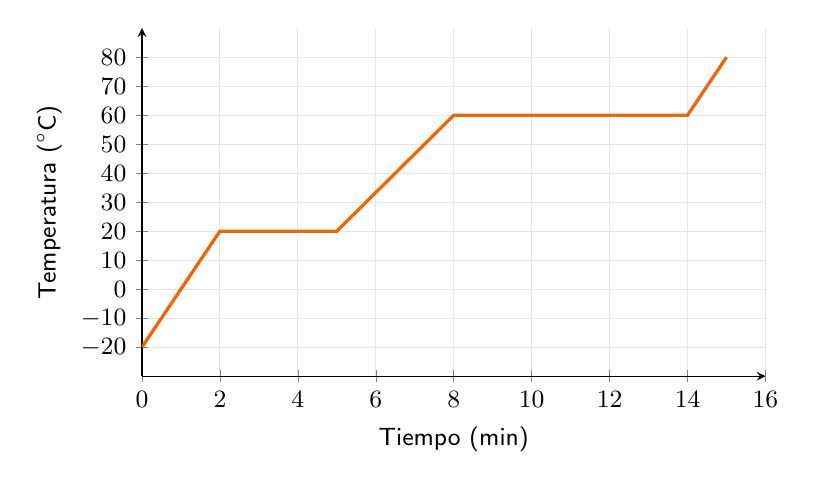
\begin{tikzpicture}[font=\small]
\begin{axis}[axis lines=left,grid=major,grid style={gray!20},xlabel={Tiempo (min)},ylabel={Temperatura ($^\circ$C)},width=9.5cm,height=6cm,xmin=0,xmax=16,ymin=-30,ymax=90,ytick={-20,-10,0,...,80},xtick={0,2,...,16}]
\addplot[nar,very thick] coordinates {(0,-20)(2,20)(5,20)(8,60)(14,60)(15,80)};

\end{axis}
\end{tikzpicture}
\end{document}
